\documentclass[conference]{IEEEtran}
\IEEEoverridecommandlockouts
% The preceding line is only needed to identify funding in the first footnote. If that is unneeded, please comment it out.
\usepackage{cite}
\usepackage{amsmath,amssymb,amsfonts}
\usepackage{algorithmic}
\usepackage{graphicx}
\usepackage{textcomp}
\usepackage{xcolor}
\usepackage{booktabs}
\usepackage{tikz}
\usepackage{pgfplots}
\def\BibTeX{{\rm B\kern-.05em{\sc i\kern-.025em b}\kern-.08em
		T\kern-.1667em\lower.7ex\hbox{E}\kern-.125emX}}
\begin{document}
	
	\title{Integrating Neural Networks into Resource-Constrained IoT Devices: Challenges and Techniques}
	
	\author{\IEEEauthorblockN{Muhammad Saad Azam}
		\IEEEauthorblockA{\textit{Department of Computer Science} \\
			\textit{University of Engineering and Technology}\\
			Lahore, Pakistan}}
	
	\maketitle
	
	\begin{abstract}
		With the rapid increase of number of IoT devices, there has been a growing demand for intelligent lightweight devices. However, the constraints of energy, memory and computation of microcontroller-class devices make the deployment of efficient neural networks fundamentally challenging. This survey provides a structured analysis of techniques that can bridge this gap, organized across three dimensions: lightweight neural network architectures, model compression techniques and inference frameworks. We examine the tradeoffs of each architecture and if those architectures are IoT friendly. Our analysis shows that architectures like MCUNet and MCUFormer, that target both the design as well as the inference are most well-suited for IoT devices. When it comes to compression techniques, all the techniques target different paradigms of compression: Quantization universally benefits IoT devices, Knowledge Distillation (KD) is quite prominent for transformer compression, and NAS has its place for the design of the model itself, where it is more mature and prominent for CNN architectures. The frameworks are analyzed on the basis of memory, portability and execution model and how well-suited are they for MCU-class devices. Lastly, four major challenges are addressed: the memory-accuracy tradeoff, on-device continual learning, transformer deployment gap and hardware limitations for IoT devices.
	\end{abstract}
	
	\begin{IEEEkeywords}
		TinyML, microcontroller deployment, neural network compression, 
		lightweight architectures, quantization, pruning, knowledge 
		distillation, neural architecture search, vision transformers, 
		resource-constrained IoT, inference frameworks, edge AI
	\end{IEEEkeywords}
	
	\section{Introduction}
	
	Traditional statistical machine learning models have been an integral part of IoT device infrastructure. These models are generally memory-efficient, computationally inexpensive, and capable of achieving accurate predictions in many practical scenarios. Due to these characteristics, they have historically been preferred for deployment in resource-constrained IoT environments. Among these statistical models, Random Forest classifiers and similar decision forest methods have consistently performed well for a variety of IoT tasks. These models are particularly effective in scenarios where the available datasets are relatively small, as they tend to remain robust even when training data is limited \cite{meidan2017, sliwa2024}. When the underlying data is simple, well-structured, and easily interpretable, such models are often more than sufficient for achieving reliable performance in IoT applications.
	
	However, these traditional machine learning models often struggle to learn complex representations when the underlying data itself is highly complicated. Existing literature notes that although decision forests are memory-efficient and practical for constrained environments, they remain limited in expressiveness. As a result, they frequently require dynamic adaptations, such as pruning strategies or meta-learning mechanisms, in order to handle more complex patterns and concept drift in data streams \cite{lourenco2025}. Similar limitations can be observed in other statistical machine learning models that rely heavily on handcrafted features and relatively shallow model structures. Furthermore, when the input data becomes high-dimensional or unstructured—such as visual, auditory, or multimodal data—these statistical models often fail to scale effectively, which significantly restricts their ability to capture deeper patterns within the data \cite{zhou2024}.
	
	This is precisely the domain in which neural networks excel. Neural networks (NNs) are capable of learning complex hierarchical representations directly from raw data, enabling them to model intricate relationships that traditional statistical models often fail to capture. In addition, neural networks demonstrate strong scalability with respect to both the number of model parameters and the size of the datasets used during training \cite{hestness2017}. Their representational power is further enhanced through the use of activation functions that introduce non-linearity into the learning process. Moreover, various architectural innovations like Convolutional Neural Networks (CNNs) for visual data \cite{lecun1998} and Transformer architectures for sequence modeling \cite{vaswani2017} have significantly expanded the ability of neural networks to learn, generalize, and perform effectively across a wide range of complex tasks. As a result, neural networks have become a dominant approach for processing high-dimensional and unstructured data generated by modern IoT systems.
	
	However, despite their potential, there are certain challenges that are prominent with neural networks. Efficient NNs are usually large \cite{kaplan2020} and therefore cannot be efficiently integrated to lightweight, hardware-restricted IoT devices. IoT devices typically have limited memory, storage and battery life. They also lack powerful processors and GPUs. Furthermore, raw data transfer between cloud, routers and IoT devices can be expensive as well. This greatly discourages integration of NNs in IoT devices and reduces their practical utility. As a result, substantial research efforts have been made to effectively integrate NNs in lightweight IoT devices.
	
	\begin{figure*}[t]
		\centering
		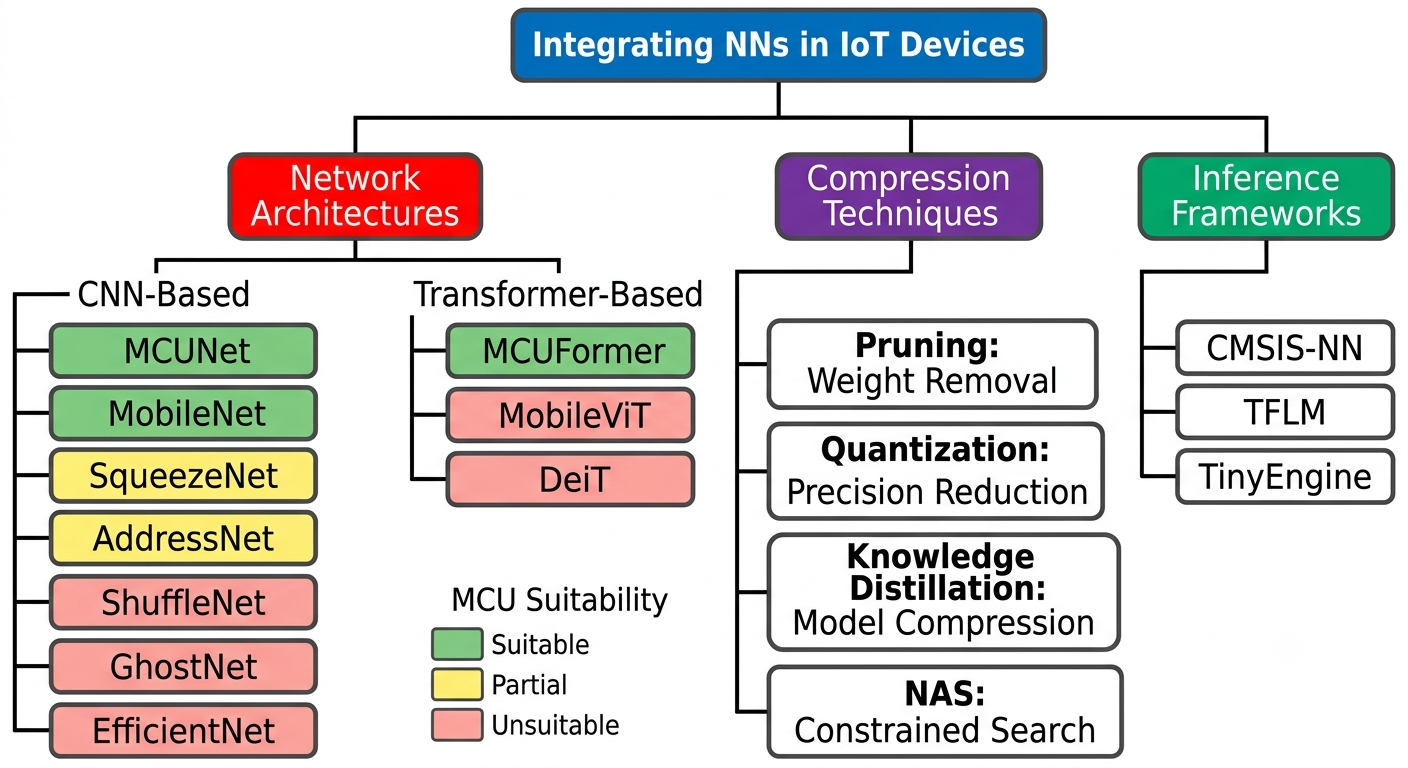
\includegraphics[width=0.9\textwidth]{./overview.png}
		\caption{Survey Overview}
		\label{fig:overview}
	\end{figure*}
	
	
	Numerous developments have been made for lightweight integration of deep learning in resource-constrained environments, targeting different aspects of the deep learning ecosystem like hardware, network architecture, deployments and more \cite{liu2024}. However, memory, performance, and hardware constraints of IoT devices make this integration considerably more challenging, and further research is required to address these gaps in a unified manner. This survey attempts to fill that gap.
	
	\section{IoT Landscape and Constraints}
	
	\subsection{Device Tiers}
	Based on the tasks and their capabilities, we are going to divide IoT devices into three tiers. Each tier varies in capability and serves a distinct role in the overall IoT architecture..
	
	\subsubsection{Tier 1: Ultra-constrainted Microcontrollers}
	These IoT devices have the smallest SRAM and flash memory. The SRAM typically ranges from 16 to 512kb while flash storage is typically less than 2MB. The power consumption is less than 1mW in active mode and have no operating systems. Device families like ARM Cortex M0/M0+, ultra low-power NPU and RISC-V ultra-constrained MCUs come under this tier. The TinyML framework primarily targets devices under this tier \cite{lin2023}.
	
	\subsubsection{Tier 2: Capable Processors}
	Devices like Raspberry Pi, Nvidia Jetson Nano, and ARM Cortex-A based SOCs can be categorized under this tier. The RAM ranges from hundred megabytes to a few gigabytes with optional hardware accelerators. These devices allow to us to deploy and infer deep learning models that are more accurate and efficient. Such devices can run minimal operating systems like RIOT OS \cite{baccelli2018}. Models like MobileNet and ResNet can be used for inference on these devices.
	
	\subsubsection{Tier 3: Edge Servers and Gateways}
	Devices within this tier represent the most capable class of hardware, typically offering gigabytes of memory, substantial storage capacity, and highly efficient high-performance processors. These platforms are capable of running full-scale deep learning models, including convolutional neural networks (CNNs) and transformer-based architectures. Commonly deployed in edge AI systems and cloud-connected infrastructures, they often serve as aggregation points for data collected from lower-tier IoT devices. They are also able to run operating system like Linux. As these devices are already capable of running heavy models, these devices are not a primary focus of this survey.
	
	In a typical IoT architecture, all these devices intercommunicate with each other. Among the hardware tiers discussed, ultra-constrained microcontrollers present the greatest challenges for deep learning deployment because of their severe limitations in memory, storage, processing capability, and energy availability. As a result, much of the recent research in TinyML, embedded AI, and resource-aware model optimization has focused specifically on enabling intelligent inference on these highly constrained devices.
	
	\begin{figure}[h]
		\centering
		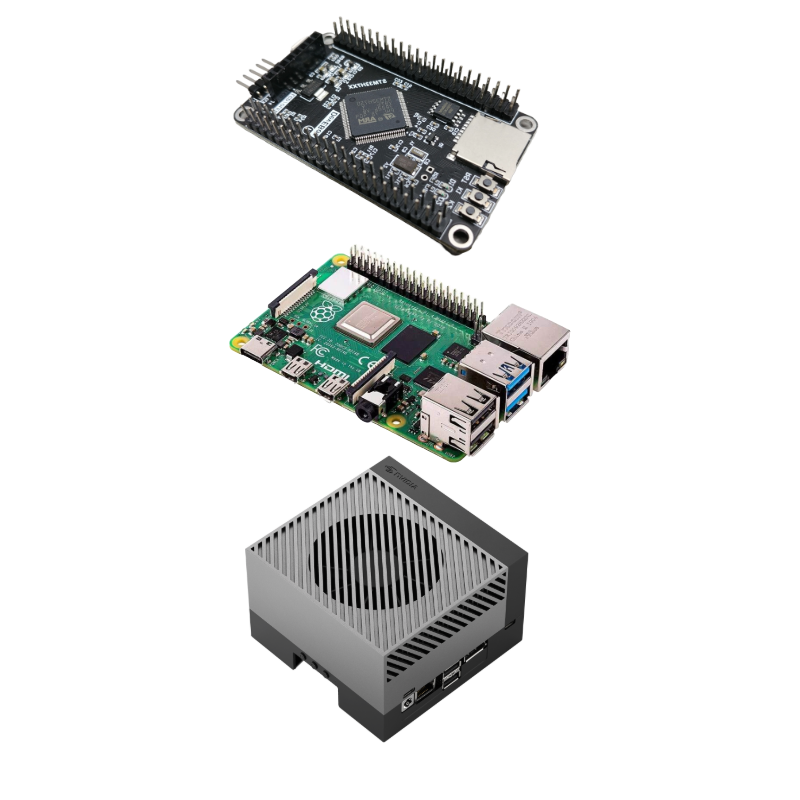
\includegraphics[width=0.5\textwidth]{../papers/assets/devices.png}
		\caption{Device of each tier. 1st one is STM32, 2nd Raspberry PI 4, and 3rd is Nvidia Jetson AGX Orin}
		\label{fig:devices tier}
	\end{figure}
	
	\subsection{Key Constraints}
	IoT devices operate under several fundamental constraints that complicate neural network deployment:
	
	\subsubsection{Memory} SRAM is the dominant bottleneck. Ultra-constrained MCUs rely solely on SRAM for computation. Standard deep learning models generate activation tensors that can easily exceed SRAM capacity.
	\subsubsection{Computation} MCUs (Microcontroller Units) usually have a clock cycle of 48MHz to 480MHz and limited instruction parallelism. This forces our hand to carry out MAC (multiply-accumulate) more efficiently within limited constraints. Architectures like SqueezeNet \cite{squeezenet2016} and MobileNet \cite{mobilenet2017} can reduce the number of operations, making such compressed architectures more suitable for IoT devices.
	\subsubsection{Energy} Most IoT deployments utilize battery-powered or energy-harvesting devices that impose strict power budget. Energy consumption during inference and training depends on the memory, numerical precision and arithmetic computation. Furthermore, DRAM consumes way more energy per bit compared to SRAM.
	\subsubsection{Numerical Precision} Typically, models use 32-bit precision floating points but that consumes a lot of SRAM. To fit such models within microcontrollers, some kind of compression is required. Quantization and pruning can help us out here, with a trade-off being the accuracy of those models.
	\subsubsection{Storage} The weights of the model reside in a flash memory, where a typical flash memory consists of 512kb to 8MB. Models like ResNet-50 \cite{resnet2016} requires around 98MB of storage with float32 precision. Quantization to 4-bit compresses the size to 12MB which is still a lot for MCUs. Hence, pruning and low-bit quantization is an important requirement for compression.
	\subsubsection{Latency} Most of the IoT devices for anomaly, object and gesture detection require a response of milliseconds. Hence, the models deployed should meet the real-time requirements of these IoT devices, with quick inference and minimal latency.
	
	\section{Implementation Strategies}
	Based on these constraints, the implementation, optimization, and deployment of deep learning models can be approached from multiple directions. The key areas of focus include neural network architectures, model compression strategies, hardware advancements and their suitability for AI integration, as well as lightweight frameworks that enable efficient deployment of AI on MCUs.
	
	In this survey, we analyze these strategies in terms of their computational complexity and suitability for MCU deployment. We further examine the trade-offs between computation, memory usage, performance, and accuracy to identify practical operating points and highlight any standout approaches. Existing benchmarks are catalogued based on their computational requirements, performance, and accuracy trade-offs, with the analysis conducted primarily through the lens of IoT devices.

	\section{Network Architecture}
	Our first area of interest in network architecture, where various neural networks of different compositions are introduced. Some architectures excel in accuracy while others chiefly focus on performance with minimal parameters. When it comes to vision tasks, CNNs are competent on lightweight IoT devices, providing a favorable balance between performance and accuracy. However, since the introduction of transformer architecture \cite{vaswani2017}, vision transformers have gathered a lot of attention and growing amount of research is being done to make them more lightweight and efficient. First, we outline models utilizing CNN architecture, their trade-offs and then the vision transformers.
	
	\subsection{Lightweight CNNs}
	
	\subsubsection{SqueezeNet}
	SqueezeNet was introduced in 2016 with the goal of matching AlexNet's \cite{alexnet2012} performance with greatly reduced parameter count with minimal memory footprint \cite{squeezenet2016}. SqueezeNet achieves this reduction by using $1\times1$ convolution filters instead of $3\times3$ convolutions. The squeeze layers reduce the number of input channels to subsequent filters. The resulting model has a memory footprint of approximately 4.8MB. This model can be further compressed with deep compression \cite{han2015} (pruning, quantization to 6-bit and huffman coding), resulting in a light 0.48MB model. This deep compression achieved comparable performance to the uncompressed one. While uncompressed SqueezeNet is not suitable for MCUs, there have been deployments of SqueezeNet-like CNNs on microcontrollers like Arduino Portenta H7 Lite \cite{lillo2024}, making SqueezeNet-inspired architectures a potential candidate for tier 1 devices.
	
	\subsubsection{ShuffleNet}
	ShuffleNet achieves reduction in model parameters and computation (FLOPs) by using group convolution and channel shuffling \cite{shufflenet2017}. Instead of connecting every input channel to output channel, channels are split into groups which greatly minimizes computation and parameters. However, because of this grouping, each group sees its own channel which results in loss of information as there is no cross-mixing of the channels. To compensate, the channels are shuffled in the groups. Because of these operations, minimum accuracy is lost with reduction in computation and parameters. Because of this optimization, ShuffleNet is a strong candidate among IoT devices because of low FLOPs and storage requirement, especially the quantized and pruned versions.
	
	\begin{table*}[h]
		\centering
		\caption{Comparison of lightweight CNN models for MCU deployment}
		\label{tab:model_comparison}
		\resizebox{\textwidth}{!}{%
			\begin{tabular}{|l|c|c|c|c|c|l|}
				\hline
				Model & Year & Parameters & Top-1 Acc. (ImageNet) & Memory (MB) & MCU Deployed? & Evidence \\
				\hline
				SqueezeNet \cite{squeezenet2016} 								 & 2016 & 1.25M & 57.5\% & 4.8 & No & No MCU deployment found \\
				SqueezeNet (deep compressed) \cite{squeezenet2016} & 2016 & 1.25M & 57.5\% & 0.47 & Yes & \cite{lillo2024} \\
				ShuffleNet v1 \cite{shufflenet2017} 								 & 2017 & $\sim$1.42M\textsuperscript{a} & 67.6\% & $\sim$7.5 & No & ARM mobile CPU only \cite{shufflenet2017} \\
				MobileNet v1 1.0 \cite{mobilenet2017} 							  & 2017 & 4.2M & 70.6\% & $\sim$16.8 & No & No MCU deployment found \\
				AddressNet-20 \cite{addressnet2018} 							& 2018 & 0.08M & 68.68\% & $\sim$0.32 & No &  No MCU deployment found \\
				MobileNet v1 (mixed precision) \cite{rusci2019} 			 & 2019 & 4.2M & 68.0\% & $\sim$2.0 & Yes & STM32H743 \cite{rusci2019} \\
				EfficientNet-B0 \cite{efficientnet2019}								& 2019 & 5.3M & 76.3\% & $\sim$21.2 & No & Too large for MCUs \\
				GhostNetV1 \cite{ghostnet2020}										& 2020 & 5.2M & 75.7\% & $\sim$20.8 & No & Too large for MCUs \\
				MCUNet (4-bit) \cite{mcunet2020}								   & 2020 & $\sim$4M & 70.7\% & 1.9 & Yes & STM32 Family \cite{mcunet2020} \\
				MCUNetV2 (8-bit) \cite{mcunet2021}							     & 2021 & - & 71.8\% & $\sim$2 & Yes & STM32 Family \cite{mcunet2021} \\
				MNv4-Conv-S \cite{mobilenet2024} 								 & 2024 & 3.8M & 73.8\% & $\sim$15.2 & No & Primarily for mobile CPUs/GPUs \\
				MCUFormer \cite{mcuformer2023}									& 2023 & - & 73.62\% & 0.32 & Yes & STM32F746 \cite{mcuformer2023} \\
				\hline
			\end{tabular}%
		}
		\begin{minipage}{\textwidth}
			\centering
			\vspace{0.5em}
			\footnotesize
			\textsuperscript{a} Estimated from architecture table \cite{wolframshufflenet}; not reported in \cite{shufflenet2017}.\\
		\end{minipage}
	\end{table*}
	
	\begin{figure*}[t]
		\centering
		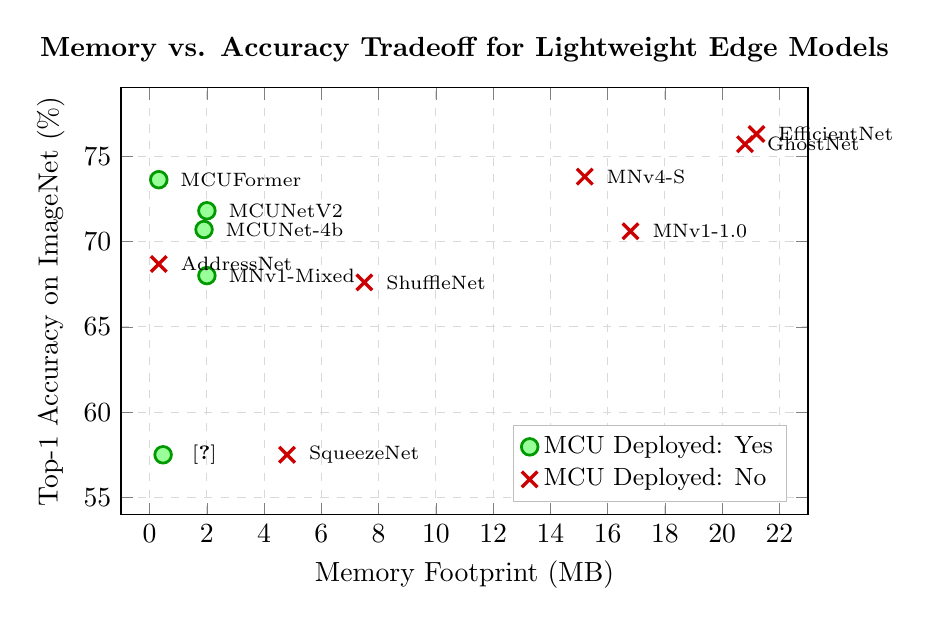
\begin{tikzpicture}
			\begin{axis}[
				width=0.85\textwidth,
				height=7cm,
				xlabel={Memory Footprint (MB)},
				ylabel={Top-1 Accuracy on ImageNet (\%)},
				title={\textbf{Memory vs. Accuracy Tradeoff for Lightweight Edge Models}},
				xmin=-1, xmax=23,
				ymin=54, ymax=79,
				grid=both,
				grid style={dashed, gray!30},
				legend pos=south east,
				legend cell align={left},
				legend style={font=\small, draw=gray!50},
				nodes near coords,
				point meta=explicit symbolic,
				every node near coord/.append style={
					font=\scriptsize, 
					color=black,
					anchor=west,
					xshift=4pt
				}
				]
				
				% Group 1: MCU Deployed = Yes (Green Circles)
				\addplot[
				only marks,
				mark=*,
				mark size=3pt,
				color=green!60!black,
				fill=green!40,
				line width=1pt
				] table[meta=label] {
					x   y   label
					0.47 57.5 {\cite{lillo2024}}
					2.0  68.0 {MNv1-Mixed}
					1.9  70.7 {MCUNet-4b}
					2.0  71.8 {MCUNetV2}
					0.32 73.62 {MCUFormer}
				};
				\addlegendentry{MCU Deployed: Yes}
				
				% Group 2: MCU Deployed = No (Red Crosses)
				\addplot[
				only marks,
				mark=x,
				mark size=4pt,
				color=red!80!black,
				line width=1.2pt
				] table[meta=label] {
					x   y   label
					4.8  57.5 {SqueezeNet}
					7.5  67.6 {ShuffleNet}
					16.8 70.6 {MNv1-1.0}
					0.32 68.68 {AddressNet}
					21.2 76.3 {EfficientNet}
					20.8 75.7 {GhostNet}
					15.2 73.8 {MNv4-S}
				};
				\addlegendentry{MCU Deployed: No}
				
			\end{axis}
		\end{tikzpicture}
		\caption{Experimental tradeoff mapping between volatile/non-volatile memory requirement and ImageNet top-1 precision. Green markers represent successful bare-metal or microcontroller deployments, while red markers indicate models that violate standard MCU physical memory thresholds.}
		\label{fig:memory_accuracy_tradeoff}
	\end{figure*}
	
	
	\subsubsection{MobileNet}
	The MobileNet series of models is a lightweight architecture of Neural Networks that achieved high accuracy by reducing the computation at inference and lowering the number of parameters \cite{mobilenet2017}. The core innovation of this architecture came from separation of spatial filtering and channel mixing using small filters, which resulted in high accuracy with reduced computation and size. Compared to SqueezeNet, the amount of FLOPs (Floating Point Operations) is greatly reduced in MobileNet which makes it even more suitable for lightweight devices with deep compression, as it has been deployed to MCUs like STM32H7 \cite{rusci2019}. The latest release of MobileNetv4 further enhanced the accuracy by utilizing Universal Inverted Bottleneck (UIB) and Mobile Multi-Query Attention (MQA) \cite{mobilenet2024}
	
	\subsubsection{AddressNet}
	In the paper of AddressNet, two limitations are highlighted of other CNN architectures; MobileNet and ShuffleNet. It states that the shuffling of channels in ShuffleNet uses zero FLOPs but still consumes 24\% of the inference time, and MobileNet's depthwise convolution takes up 20\% of inference time, despite using less parameters \cite{addressnet2018}. To overcome this latency, AddressNet introduces pointer shifts instead of direct memory shifts. This greatly reduces the expensive memory access, decreasing the inference time. This pointer shifting can be done for channel shuffling. Furthermore, AddressNet replaces depthwise convolution by shifting the pointer of the feature map in four directions (up, down, left, right). While AddressNet is not used directly in MCUs, variants and different modifications over this architecture have shown great potential.
	
	\subsubsection{EfficientNet}
	Earlier, the CNN architecture focused on making it wider, deeper or using high resolution images for input. Instead of focusing on only one dimension, EfficientNet argues to scale along all the dimensions in a balanced manner \cite{efficientnet2019}. This balance helps achieve reduced parameter size, better inference and higher accuracy. Similar to other architectures, vanilla EfficientNet is not suitable for MCU deployment but quantized and pruned versions are viable for microcontrollers with minimum accuracy loss.
	
	\subsubsection{GhostNet}
	The authors of GhostNet observed that many of the feature maps learned by CNNs are redundant. Instead of using standard convolution to compute those feature maps, they introduced 'ghost modules' by simple linear transformations of existing feature maps with minimal information loss. This transformation keeps the computation and number of parameters reduced while achieving competent accuracy to that of MobileNetV3 \cite{ghostnet2020}. However, original GhostNet models are relatively large for microcontrollers. Pruning and quantization are a necessity to make them microcontroller feasible.
	
	\subsubsection{MCUNet}
	Instead of treating inference engine and neural network architecture as two separate tasks, MCUNet designs both the system as well as the model \cite{mcunet2020}. MCUNet introduces TinyNAS (Tiny Network Architecture Search) and TinyEngine. TinyNAS optimizes the search space itself based on the hardware - input resolutions, width multipliers, kernel sizes and other architecture options. TinyEngine is the inference engine. Unlike TensorFlow Lite Micro and other frameworks that have big overhead as they are interpreter-based, TinyEngine compiles the exact model instead of interpreting it at runtime. This reduces SRAM, flash overhead and latency. With these optimizations and quantization, MCUNet is easily deployable on microcontrollers. MCUNet was the first neural network on microcontroller to achieve more than 70\% accuracy on ImageNet Top-1 classification. The latest release in MCUNet series is MCUNetV2 which further improves the memory consumption and other parameters of vanilla MCUNet, making it more lightweight as well as more accurate \cite{mcunet2021}.
	
	\subsection{Transformers}
	
	The transformer architecture has demonstrated considerable potential across vision tasks since its introduction \cite{vaswani2017}. It has shown good understanding of context and images, even showcasing improved results over CNN architecture. However, one of the overarching limitations of transformers is their heavy computation and data requirement, something that is quite challenging to deploy on resource-constrainted IoT devices. Some efforts have been made to make them lighter and more IoT friendly.
	
	\subsubsection{DeiT}
	Data efficient image transformers (DeiT) is one of the earliest attempts to make a lightweight transformer model on ImageNet \cite{deit2021}. With 86M parameters, DeiT achieved a top-1 accuracy of 83.1\%. Furthermore, a distilled model was also prepared where the student learns from the teacher via attention and the student model actually achieved better performance, with an accuracy of 85.2\%. While, the results show promise for VITs, 86M parameters is too much for IoT devices which usually have quite small flash storage and processing power. But DeiT did show us that transformers can compete with the CNN architecture.
	
	\subsubsection{MobileViT}
	With the goal of preparing smaller vision transformers and combining the strengths of CNN architecture with transformers, MobileViT is introduced \cite{mobilevit2022}. Compared to DeiT, MobileViT treats the transformer layers as convolutional layers, uses substantially fewer parameters (around 6M) and achieved better accuracy than MobileNetv3 (with a top-1 accuracy of 78.4\%, 3.2\% better than MobileNetv3). While 6M is still not quite manageable for small IoT devices, it is definitely a good development towards integration of transformers in IoT devices.
	
	\subsubsection{MCUFormer}
	Probably one of the most successful and practical integration of vision transformers in IoT devices, MCUFormer optimized the implementation in both design as well as inference \cite{mcuformer2023}. When it comes to architecture, MCUFormer one-shots NAS to find an optimized architecture from a huge search space of subnets, in an attempt to find an ideal setup without sacrificing major performance. When it comes to inference, despite minimal architecture, standard inference engines duplicate intermediate activation tensors, consuming more SRAM. MCUFormer tackles this issue by operator integration (fusing), patch embedding decomposition and token over-writing, greatly reducing the SRAM requirement \cite{mcuformer2023}. MCUFormer reports top-1 accuracy of 73.62\% on ImageNet with 320KB memory on STM32F746 microcontroller. MCUFormer highlights how ViTs can still be made NAS-friendly and how we can optimize the memory footprint during inference.
	
	\section{Compression Techniques}
	
	\subsection{Pruning}
	Pruning removes neurons, filters or even entire layers that are doing little for the neural network. The intuition being, neural networks are usually quite dense where most of the neurons are either redundant or doing barely anything for efficiency of the network. Pruning tries to remove those redundant weights, weak neurons and unimportant channels.
	
	The earliest implementation of pruning involved calculating second order derivates to approximate the unimportant neurons and then removing them from the network \cite{pruning1990}. One limitation in this approach is that the weights are reduced at initialization, making the removal of weights a little less justified. However, post-training pruning has been quite successful \cite{pruning2015}. In this technique, a neural network is first trained and then later on weights are removed without major sacrifices to accuracy. Then, the remaining network is re-trained for more robustness. These approaches highlighted come under the category of unstructured pruning, where individual weights are removed irrespective of their position in the tensor. This creates irregularities in connectivity and hardware improvements are limited.
	
	On the other hand, structural pruning removes entire structural units of the neural network, like filters or channels in CNNs or fully connected layers in DNNs (Dense Neural Networks). Because of entire removal of structural units, the sanctity of the structure remains and we gain boost in hardware performance without any special sparse kernels. Early implementations of structural pruning involve removing filters that are less significant, based on the criteria of L1 norm \cite{structuralpruning2017}.
	
	Extensive analysis has been carried out to understand the impact of pruning on NNs. One hypothesis synthesizes that pruning can reduce the size of the network by 80 to 90\% without sacrificing accuracy where specific modules have won 'the lottery ticket'. When a similar sized network is trained in isolation, the performance is worse. So, the lottery won by pruned model lies in the initialization of the neural network \cite{lotteryhypothesis2019}. This hypothesis has directed the research for pruning, where finding 'the lottery ticket' has become a focus before after initialization and before training \cite{synflow2020}.
	
	Pruning is one of the most prominent technique to make neural networks more microcontroller feasible. It has been used in conjunction with quantization and huffman coding to aggressively reduce model sizes \cite{han2015}. Heavier model architectures like MobileNet and SqueezeNet have been pruned and deployed to MCUs \cite{lillo2024}.
	
	\subsection{Quantization}
	Quantization is the most prominent technique of greatly minimizing the model size by quantizing the data type of the neural network to less precision. For high accuracy, neural networks typically use single-precision 32-bit floating point (FP32) for weights. However, FP32 constitutes of 4 bytes. So, a model of 5M parameters is going to take up 20MB of storage, which is not viable for microcontrollers at all. Here, quantization comes into play, where the weights are quantized to a lower precision data type like INT8, INT4 etc, greatly reducing the model size.
	
	The earlier impact of quantization can be seen in BinaryConnect, which showed that weights constrained to only -1 or +1 at extremely low precision can work for neural networks \cite{binarynet2015}. One of the influential studies and breakthrough in quantization was achieved by quantizing the floating points to integers \cite{quantization2018}. Floating points have shown to be more compute intensive and slower at inference. But with integers, if done properly, quantization can achieve great reduction in model size without any major sacrifices to accuracy. The authors also introduced Quantization-Aware Training (QAT). Early implementation of quantization will take a model and quantize the learned weights later, which results in greater accuracy drops. With QAT, the model 'simulates' the impact of quantization in the forward pass. This makes models like MobileNet and EfficientNet more microcontroller friendly \cite{quantization2018, han2015, lillo2024, mcunet2020, mcunet2021}. Integer-only quantization has become mainstream for TinyML and frameworks like TensorFlow-Lite. Mixed-precision quantization is also used for even lesser drops in accuracy, where some layers can use high-precision quantized integers while others utilize low-precision weights \cite{rusci2019}.
	
	Quantization is easily one of the most extensively used technique to lower the memory footprint of neural networks, increase hardware access and make inference faster, with minimal drops in accuracy.
	
	\begin{table*}[h]
		\centering
		\caption{Comparison of Model Compression Techniques for TinyML/IoT Deployment}
		\label{tab:compression}
		\renewcommand{\arraystretch}{1.3}
		\begin{tabular}{|p{2.8cm}|p{3cm}|p{2.8cm}|p{3cm}|p{2.5cm}|}
			\hline
			\textbf{Technique} & \textbf{Compression Target} & \textbf{Suitability for MCUs} & \textbf{Compression Aggressiveness} & \textbf{Accuracy Impact} \\
			\hline
			\textbf{Pruning} (Unstructured) & Individual weights \& neurons & Moderate — requires sparse kernel support & High (80--90\% weight removal possible) & Low to moderate \\
			\hline
			\textbf{Pruning} (Structural) & Filters, channels, entire layers & High — preserves tensor structure; hardware-friendly & Moderate & Low to moderate \\
			\hline
			\textbf{Quantization} & Weight \& activation precision (FP32 $\rightarrow$ INT8/INT4) & Very High — natively supported on MCUs; mainstream in TFLite & Very High (4$\times$--8$\times$ size reduction) & Minimal (esp. with QAT) \\
			\hline
			\textbf{Knowledge Distillation} & Model capacity \& architecture & High — produces lightweight student models & Moderate (bounded by student architecture) & Low (often improves generalisation) \\
			\hline
			\textbf{NAS} & Network architecture design & High — can target IoT/energy constraints explicitly & Moderate to High (architecture-dependent) & Low (optimised by design) \\
			\hline
		\end{tabular}
	\end{table*}
	
	\subsection{Knowledge Distillation}
	In Knowledge Distillation (KD), a larger model (called the teacher) trains a smaller model (called the student) using its own internal representations. This is one of the most used technique to train high accuracy, small lightweight IoT devices. KD was introduced in 2014, with the idea that teacher model learns the hard target labels and reasons about it in soft probabilities. The student model then not only learns the 'softer' representations of the teacher, but also the hard labels, making it more concise and rich in learning \cite{knowledgedistillation2014}. This often achieves better convergence, generalization and robustness. While the student learns the output probabilities from the teacher, other approaches learn different parameters from the teachers. For example, FitNets extend the idea of classic KD where the student model learns not only the output probabilities but also the intermediary representations of the teacher \cite{fitnets2015}.
	
	Since then, there have been new variations of distillations introduced. In online distillation, teacher and student models are trained in conjunction, compared to classic distillation where teacher is trained first \cite{deepmutuallearning2018}. In self-distillation, the teacher trains itself by using its own soft targets. The soft targets act as smoothening representations that improve the accuracy of the model, making it more 'intelligent' \cite{selfdistilliation2019}. 
	
	\subsection{Network Architecture Search (NAS)}
	NAS was introduced in 2016 as a way to generate neural network architectures using a neural network controller trained with reinforcement learning. While the original showcased promising and efficient architectures, the computation cost was enormous for a single search \cite{nasrl2017}. To optimize the search space, two major breakthroughs emerged: DARTS (Differentiable Architecture Search) which made NAS more continuous and less discrete, immensely optimizing the search space \cite{darts2019} and PNAS (Progressive Neural Architecture Search) which sequentially made improvements over the model, improving the design and efficiency of the model without requiring the big search cost of vanilla NAS \cite{pnas2018}.
	
	Since the introduction of NAS, the research has now also expanded to design neural networks more IoT friendly and energy aware. Energy-aware NAS addresses the energy cost of deploying DNNs on lightweight devices, and attempts to design best performing lightweight Dense Neural Networks that are subjected to IoT constraints \cite{energyawarenas2024}. TinyFusion-NAS is a hardware-aware NAS which targets deployment of lightweight attention to small sensor based IoT devices within the smallest constraints \cite{tinyfusionnas2026}
	
	While NAS is quite mature in the form of DARTS and PNAS, it is not well-suited for transformers. The earliest experiment of NAS over vision transformers is NASViT \cite{nasvit2022}. However, it quickly highlighted the gradient conflict problem where gradients of different subnetworks conflict with the supernet more severely in ViTs than CNNs, leading to early saturation and inferior convergence. Other work reasoned about this differently, citing the channel imbalance because of the token embeddings \cite{vitas2021}. There have been more attempts to counter these challenges, like DASViT (a DARTS-like NAS for ViTs) \cite{dasvit2025} and OoD-ViT-NAS (focused on out-of-distribution generalization) \cite{oodvitnas2024}.
	
	\section{Frameworks}
	
	Deploying neural networks on IoT devices requires not only optimized model architectures and compression techniques, but also an inference runtime that can operate within the severe memory, storage, and compute constraints of microcontrollers. The frameworks discussed below span two distinct paradigms: low-level kernel libraries that accelerate individual operations and higher-level inference engines that manage the full model execution pipeline.
	
	\subsection{CMSIS-NN}
	
	CMSIS-NN (Cortex Microcontroller Software Interface Standard for Neural Networks) is a low-level collection of optimized neural network kernels developed by ARM, specifically targeting Cortex-M processors \cite{cmsisnn2018}. It is not a full inference engine but rather a hardware-optimized backend that helps in boosting operations like convolution, pooling, fully connected layers, and activation functions. The library is organized into two components: NNFunctions, which provides the core operator kernels, and NNSupportFunctions, which provides utility functions such as data conversion and activation lookup tables that can be composed into more complex modules like LSTMs and GRUs \cite{cmsisnn2018}.
	
	The key optimization in CMSIS-NN lies in its exploitation of SIMD (Single Instruction, Multiple Data) capabilities available in ARMv7E-M and ARMv8-M processors. It leverages 16-bit MAC instructions to perform two MAC operations in a single 32-bit accumulator cycle, effectively doubling arithmetic throughput. The library supports both INT8 and INT16 quantized operations, avoiding costly floating-point computation and reducing the memory footprint of activations and weights—both of which are critical for SRAM-constrained MCUs \cite{cmsisnn2018}. Benchmarks show that inference using CMSIS-NN kernels achieves a 4.6$\times$ improvement in runtime throughput and a 4.9$\times$ improvement in energy efficiency compared to baseline implementations using standard DSP operations \cite{cmsisnn2018}.
	
	CMSIS-NN is not a standalone deployment solution. Rather, it is designed to be used as an optimized backend for higher-level frameworks. Notably, TensorFlow Lite Micro (TFLM) integrates CMSIS-NN as its hardware acceleration layer for ARM targets, and the library maintains bit-exact equivalence with TFLM reference kernels \cite{cmsisnn_github}. Models like MobileNet with mixed-precision quantization have been deployed on STM32 microcontrollers making direct use of CMSIS-NN kernels \cite{rusci2019}. Because CMSIS-NN is ARM-specific, it does not offer portability to other architectures such as RISC-V without significant modification, which remains one of its central limitations.
	
	\subsection{TensorFlow Lite Micro (TFLM)}
	
	TensorFlow Lite Micro (TFLM) is an open-source inference framework developed by Google for deploying neural networks on deeply resource-constrained embedded devices \cite{tflm2021}. TFLM is a specialized derivative of TensorFlow Lite, stripped of features that are impractical on MCUs—such as dynamic memory allocation, operating system dependencies, and standard C library reliance—while retaining a portable, cross-platform design. Written in C++11, it requires only a 32-bit processor and is compatible with a wide range of ARM Cortex-M series processors as well as the ESP32 \cite{tflm2021}.
	
	TFLM uses an interpreter-based execution model, representing the neural network as a graph of operators and tensors. At initialization, the framework performs a one-time memory planning step that allocates a shared memory arena for all activation tensors. This eliminates runtime dynamic allocation entirely, an essential property for bare-metal MCU deployments. The framework is composed of three primary components: an operator resolver, which links only those operations required by the given model into the binary; a pre-allocated memory stack; and an interpreter that resolves the graph and dispatches operator execution \cite{tflm2021}. The interpreter footprint itself is less than 2KB, and for practical models like keyword spotting and visual wake words, total memory consumption remains well within 30KB of SRAM \cite{tflm2021}.
	
	TFLM natively integrates CMSIS-NN as a kernel backend for ARM targets, allowing operators like convolution to benefit from SIMD hardware acceleration without any changes to the user-facing API. Models trained in TensorFlow or Keras are first converted to the FlatBuffer \texttt{.tflite} format using post-training quantization—typically to INT8—and are then deployed on target hardware through the TFLM runtime. The interpreter overhead itself is minimal, at less than 0.1\% of total inference cycles for non-trivial models \cite{tflm2021}. However, the interpreter-based approach does carry one fundamental cost: the model graph metadata must reside in memory alongside the model weights, introducing overhead that is avoidable in compiler-based approaches. Furthermore, TFLM's operator coverage, while broad, does not extend to every layer type—certain operations like GRU, Conv1D, and some activation functions are not supported, limiting its applicability to a subset of neural network architectures \cite{efficientnnsreview2023}.
	
	Despite these limitations, TFLM remains the most widely adopted deployment framework for TinyML, owing to its well-maintained documentation, hardware portability, and integration with the larger TensorFlow ecosystem.
	
	
	\begin{table}[h]
		\centering
		\caption{Comparison of deployment frameworks for MCU inference}
		\label{tab:framework_comparison}
		\resizebox{\columnwidth}{!}{%
			\begin{tabular}{|l|c|c|c|}
				\hline
				Property & CMSIS-NN & TFLM & TinyEngine \\
				\hline
				Type & Kernel Library & Interpreter & Code Generator \\
				Execution Model & Kernel calls & Runtime graph & Compiled C \\
				Standalone Runtime & No & Yes & Yes \\
				INT8 Support & Yes & Yes & Yes \\
				INT4 Support & No & No & Yes \\
				OS Required & No & No & No \\
				Cross-platform & ARM only & Broad & ARM Cortex-M \\
				Peak SRAM vs TFLM & Lower & Baseline & 2.7--4.8$\times$ lower \\
				Inference Speed vs TFLM & Higher & Baseline & 1.5--3$\times$ faster \\
				Open Source & Yes & Yes & Yes \\
				\hline
			\end{tabular}%
		}
	\end{table}
	
	\subsection{TinyEngine}
	
	TinyEngine is a code generation-based inference engine introduced alongside MCUNet as part of a system-algorithm co-design approach to TinyML \cite{mcunet2020}. Unlike TFLM and CMSIS-NN, which follow an interpreter-based execution model, TinyEngine compiles the exact model into device-specific C code rather than interpreting a graph representation at runtime. This distinction has significant practical consequences: interpreter-based frameworks must store model metadata—such as tensor shapes, operator configurations, and graph connectivity—in memory at runtime, consuming SRAM that is otherwise unavailable for activations. TinyEngine eliminates this overhead entirely through code generation \cite{lin2023}.
	
	Beyond eliminating interpreter overhead, TinyEngine introduces several operator-level optimizations targeted specifically at MCU deployment. These include in-place depth-wise convolution, which reuses the input buffer for output activations to avoid double-buffering overhead, and loop reordering strategies that restructure the access patterns of convolutional operations to improve cache locality on MCUs without data caches. Additionally, TinyEngine supports operator fusion, which reduces the number of memory read-write cycles by combining consecutive operations into a single kernel pass \cite{lin2023}. Collectively, these optimizations result in TinyEngine reducing peak SRAM usage by 2.7--4.8$\times$ and improving inference speed by 1.5--3$\times$ compared to TF-Lite Micro and CMSIS-NN on identical models \cite{mcunet2020}.
	
	TinyEngine is tightly coupled to the MCUNet ecosystem: models are searched using TinyNAS with memory profiling performed through TinyEngine's code generator, ensuring that the NAS search space is directly constrained by the actual on-device memory schedule rather than theoretical estimates. This hardware-model co-design was instrumental in enabling MCUNet to achieve over 70\% ImageNet Top-1 accuracy on commercial off-the-shelf microcontrollers, a milestone that interpreter-based frameworks had not been able to reach \cite{mcunet2020}. The primary limitation of TinyEngine is its reduced portability: being a compiler-based code generator specialized for ARM Cortex-M targets, it lacks the cross-platform flexibility of TFLM, and its tighter coupling to the MCUNet model family makes adapting it to arbitrary architectures more involved.
	
	\subsection{Framework Comparison}
	
	The three frameworks occupy distinct positions in the deployment stack. CMSIS-NN is a hardware primitive library and not a standalone runtime; it is best understood as the acceleration backend upon which higher-level frameworks are built. TFLM is the most portable and widely adopted inference engine, supporting a broad range of hardware platforms and neural network operators, but at the cost of interpreter overhead and larger memory footprint compared to compiled alternatives. TinyEngine represents the state-of-the-art in memory efficiency and inference speed for MCU deployment, but trades portability and generality for that performance.
	
	\section{Challenges}
	
	While significant progress has been made when it comes to deploying neural networks by optimizing the inference, architecture and compression, there are still certain challenges yet unresolved and can be substantially improved upon.
	
	\subsection{Memory-Accuracy Tradeoff}
	The tradeoff between memory and accuracy for MCUs is largely underexplored. Each compression technique like pruning, quantization, distillation results in a collapse in accuracy after a certain point. And this threshold point is also not specified as it can deviate from task to task, or model to model. Furthermore, within these compression techniques, there are no universal indicators or benchmarks guiding the usage of these compression techniques. Lastly, the combination of the compression techniques is also underexplored.
	
	\subsection{Continual Learning}
	Within IoT devices, continual learning is still under-studied. While significant efforts have geared towards optimized inference and architecture, the on-device learning is yet to receive the attention it requires. As the sensory data and the environment for IoT devices can change significantly, continual learning and on-device training becomes even more important. And this problem is still explored in limited space. Although some efforts like MCUNetV3 attempt on-device training \cite{mcunetv32022}, many challenges remain largely unaddressed.
	
	\subsection{Hardware Limitations}
	There is no universal deployment target for IoT devices. Certain frameworks are suitable for only some subset of devices. Moreover, the standardized hardware also makes certain compression techniques more rigid. For example, while INT16, INT8 and INT4 quantizations are quite prevalent, modern hardware of NVIDIA GPUs, ARM CPUs and Apple chips is not well-suited for more continuous quantization techniques (like INT7 or INT6), which can potentially be quite beneficial for improving the memory-accuracy scores.
	
	\subsection{Transformer Deployment Gap}
	As reported earlier, there still exists a substantial gap between transformers and CNN architectures. Techniques that are mature and extensive for CNN like NAS are not transferable to vision transformers. Moreover, transformers come with other challenges like more SRAM usage, more data consumption for better accuracy, which makes inference, on-device training and deployment much more harder for transformers.
	


	\begin{thebibliography}{00}
		\bibitem{sliwa2024}
		B. Sliwa, N. Piatkowski and C. Wietfeld, "LIMITS: Lightweight Machine Learning for IoT Systems with Resource Limitations," ICC 2020 - 2020 IEEE International Conference on Communications (ICC), Dublin, Ireland, 2020, pp. 1-7, doi: 10.1109/ICC40277.2020.9149180.
	
		\bibitem{meidan2017}
		Y. Meidan, M. Bohadana, A. Shabtai, M. Ochoa, N. O. Tippenhauer, J. D. Guarnizo, and Y. Elovici, "Detection of Unauthorized IoT Devices Using Machine Learning Techniques," arXiv:1709.04647, Sep. 2017.
	
		\bibitem{lourenco2025}
		A. Lourenço, J. Rodrigo, J. Gama, and G. Marreiros, "On-device edge learning for IoT data streams: a survey," arXiv:2502.17788, Feb. 2025.
		
		\bibitem{zhou2024}
		S. Zhou et al., "A Comprehensive Survey on Deep Clustering: Taxonomy, Challenges, and Future Directions," ACM Computing Surveys, vol. 56, no. 7, pp. 1–56, Mar. 2024. DOI: 10.1145/3617813
		
		\bibitem{hestness2017}
		J. Hestness, S. Narang, N. Ardalani, G. Diamos, H. Jun, H. Kianinejad, M. M. A. Patwary, Y. Yang, and Y. Zhou, "Deep Learning Scaling is Predictable, Empirically," arXiv:1712.00409, Dec. 2017.
		
		\bibitem{lecun1998}
		Y. LeCun, L. Bottou, Y. Bengio, and P. Haffner, "Gradient-based learning applied to document recognition," Proceedings of the IEEE, vol. 86, no. 11, pp. 2278–2324, Nov. 1998.
		
		\bibitem{vaswani2017}
		A. Vaswani, N. Shazeer, N. Parmar, J. Uszkoreit, L. Jones, A. N. Gomez, L. Kaiser, and I. Polosukhin, "Attention is all you need," in Advances in Neural Information Processing Systems 30 (NIPS 2017), Long Beach, CA, USA, Dec. 2017, pp. 6000–6010.
		
		\bibitem{kaplan2020}
		J. Kaplan et al., "Scaling Laws for Neural Language Models," arXiv:2001.08361, Jan. 2020.
		
		\bibitem{liu2024}
		H.-I. Liu, M. Galindo, H. Xie, L.-K. Wong, H.-H. Shuai, Y.-H. Li, and W.-H. Cheng, "Lightweight deep learning for resource-constrained environments: A survey," ACM Computing Surveys, vol. 56, no. 7, pp. 1–42, Jul. 2024. doi: 10.1145/3657282.
		
		\bibitem{lin2023}
		J. Lin, L. Zhu, W. -M. Chen, W. -C. Wang and S. Han, "Tiny Machine Learning: Progress and Futures [Feature]," in IEEE Circuits and Systems Magazine, vol. 23, no. 3, pp. 8-34, thirdquarter 2023, doi: 10.1109/MCAS.2023.3302182.
		
		\bibitem{baccelli2018}
		E. Baccelli, C. Gündoğan, O. Hahm, P. Kietzmann, M. Lenders, H. Petersen, K. Schleiser, T. C. Schmidt, and M. Wählisch, "RIOT: An open source operating system for low-end embedded devices in the IoT," IEEE Internet of Things Journal, vol. 5, no. 6, pp. 4428–4440, Dec. 2018. doi: 10.1109/JIOT.2018.2815038.
		
		\bibitem{squeezenet2016}
		F. N. Iandola, S. Han, M. W. Moskewicz, K. Ashraf, W. J. Dally, and K. Keutzer, "SqueezeNet: AlexNet-level accuracy with 50x fewer parameters and <0.5MB model size," arXiv:1602.07360, Feb. 2016.
		
		\bibitem{mobilenet2017}
		A. G. Howard, M. Zhu, B. Chen, D. Kalenichenko, W. Wang, T. Weyand, M. Andreetto, and H. Adam, "MobileNets: Efficient convolutional neural networks for mobile vision applications," arXiv:1704.04861, Apr. 2017.
		
		\bibitem{resnet2016}
		K. He, X. Zhang, S. Ren, and J. Sun, "Deep residual learning for image recognition," in 2016 IEEE Conference on Computer Vision and Pattern Recognition (CVPR), Las Vegas, NV, USA, Jun. 2016, pp. 770–778. doi: 10.1109/CVPR.2016.90.
		
		\bibitem{alexnet2012}
		A. Krizhevsky, I. Sutskever, and G. E. Hinton, "ImageNet classification with deep convolutional neural networks," in Advances in Neural Information Processing Systems 25 (NIPS 2012), Lake Tahoe, NV, USA, Dec. 2012, pp. 1097–1105.
		
		\bibitem{han2015}
		S. Han, H. Mao, and W. J. Dally, "Deep Compression: Compressing deep neural networks with pruning, trained quantization and Huffman coding," in 4th International Conference on Learning Representations (ICLR), San Juan, Puerto Rico, May 2016.
		
		\bibitem{lillo2024}
		A. Maciá-Lillo, S. Barrachina, G. Fabregat, and M. F. Dolz, "Optimizing convolutions for deep learning inference on ARM Cortex-M processors," IEEE Internet of Things Journal, vol. 11, no. 15, pp. 26203–26219, Aug. 2024, doi: 10.1109/JIOT.2024.3393546.
		
		\bibitem{shufflenet2017}
		X. Zhang, X. Zhou, M. Lin, and J. Sun, "ShuffleNet: An extremely efficient convolutional neural network for mobile devices," arXiv:1707.01083, Jul. 2017.
		
		\bibitem{mobilenet2024}
		D. Qin, C. Leichner, M. Delakis, M. Fornoni, S. Luo, F. Yang, W. Wang, C. Banbury, C. Ye, B. Akin, V. Aggarwal, T. Zhu, D. Moro, and A. Howard, "MobileNetV4: Universal models for the mobile ecosystem," arXiv:2404.10518, Apr. 2024.
		
		\bibitem{rusci2019}
		M. Rusci, A. Capotondi, and L. Benini, "Memory-driven mixed low precision quantization for enabling deep network inference on microcontrollers," arXiv:1905.13082, May 2019.
		
		\bibitem{wolframshufflenet}
		Wolfram Research, "ShuffleNet V1 trained on ImageNet competition data," Wolfram Neural Net Repository, [Online]
		
		\bibitem{addressnet2018}
		H. Zhong, X. Liu, Y. He, and Y. Ma, "Shift-based primitives for efficient convolutional neural networks," arXiv:1809.08458, Sep. 2018.
		
		\bibitem{efficientnet2019}
		M. Tan and Q. Le, "EfficientNet: Rethinking model scaling for convolutional neural networks," in Proceedings of the 36th International Conference on Machine Learning (ICML), Long Beach, CA, USA, Jun. 2019, pp. 6105–6114.
		
		\bibitem{ghostnet2020}
		K. Han, Y. Wang, Q. Tian, J. Guo, C. Xu, and C. Xu, "GhostNet: More features from cheap operations," in *2020 IEEE/CVF Conference on Computer Vision and Pattern Recognition (CVPR)*, Seattle, WA, USA, Jun. 2020, pp. 1577–1586.
		
		\bibitem{mcunet2020}
		J. Lin, W.-M. Chen, Y. Lin, J. Cohn, C. Gan, and S. Han, "MCUNet: Tiny deep learning on IoT devices," in Advances in Neural Information Processing Systems 33 (NeurIPS 2020), Dec. 2020, pp. 1–12.
		
		\bibitem{mcunet2021}
		J. Lin, W.-M. Chen, H. Cai, C. Gan, and S. Han, "MCUNetV2: Memory-efficient patch-based inference for tiny deep learning," arXiv:2110.15352, Oct. 2021.
		
		\bibitem{deit2021}
		H. Touvron, M. Cord, M. Douze, F. Massa, A. Sablayrolles, and H. Jegou, "Training data-efficient image transformers and distillation through attention," in Proceedings of the 38th International Conference on Machine Learning (ICML), Virtual, Jul. 2021, pp. 10347–10357.
		
		\bibitem{mobilevit2022}
		S. Mehta and M. Rastegari, "MobileViT: Light-weight, general-purpose, and mobile-friendly vision transformer," in 10th International Conference on Learning Representations (ICLR), Virtual, Apr. 2022. [Online]. Available: https://openreview.net/forum?id=vh-0dUtG1j
		
		\bibitem{mcuformer2023}
		Y. Liang, Z. Wang, X. Xu, Y. Tang, J. Zhou, and J. Lu, "MCUFormer: Deploying vision transformers on microcontrollers with limited memory," in Advances in Neural Information Processing Systems 37 (NeurIPS 2023), New Orleans, LA, USA, Dec. 2023.
		
		\bibitem{pruning1990}
		Y. LeCun, J. S. Denker, and S. A. Solla, "Optimal brain damage," in Advances in Neural Information Processing Systems 2 (NIPS 1989), Denver, CO, USA, Nov. 1989, pp. 598–605.
		
		\bibitem{pruning2015}
		S. Han, J. Pool, J. Tran, and W. J. Dally, "Learning both weights and connections for efficient neural network," in Advances in Neural Information Processing Systems 28 (NIPS 2015), Montreal, QC, Canada, Dec. 2015, pp. 1135–1143.
		
		\bibitem{structuralpruning2017}
		H. Li, A. Kadav, I. Durdanovic, H. Samet, and H. P. Graf, "Pruning filters for efficient ConvNets," in 5th International Conference on Learning Representations (ICLR), Toulon, France, Apr. 2017.
		
		\bibitem{lotteryhypothesis2019}
		J. Frankle and M. Carbin, "The lottery ticket hypothesis: Finding sparse, trainable neural networks," in 7th International Conference on Learning Representations (ICLR), New Orleans, LA, USA, May 2019.
		
		\bibitem{synflow2020}
		H. Tanaka, D. Kunin, D. L. K. Yamins, and S. Ganguli, "Pruning neural networks without any data by iteratively conserving synaptic flow," in Advances in Neural Information Processing Systems 33 (NeurIPS 2020), Vancouver, BC, Canada, Dec. 2020, pp. 6377–6389
		
		\bibitem{binarynet2015}
		M. Courbariaux, Y. Bengio, and J.-P. David, "BinaryConnect: Training deep neural networks with binary weights during propagations," in Advances in Neural Information Processing Systems 28 (NIPS 2015), Montreal, QC, Canada, Dec. 2015, pp. 3123–3131.
		
		\bibitem{quantization2018}
		B. Jacob, S. Kligys, B. Chen, M. Zhu, M. Tang, A. Howard, H. Adam, and D. Kalenichenko, "Quantization and training of neural networks for efficient integer-arithmetic-only inference," in *2018 IEEE/CVF Conference on Computer Vision and Pattern Recognition (CVPR)*, Salt Lake City, UT, USA, Jun. 2018, pp. 2704–2713. doi: 10.1109/CVPR.2018.00286.
		
		\bibitem{knowledgedistillation2014}
		G. Hinton, O. Vinyals, and J. Dean, "Distilling the knowledge in a neural network," presented at the NIPS 2014 Deep Learning Workshop, Montreal, QC, Canada, Dec. 2014.
		
		\bibitem{fitnets2015}
		A. Romero, N. Ballas, S. E. Kahou, A. Chassang, C. Gatta, and Y. Bengio, "FitNets: Hints for thin deep nets," in 3rd International Conference on Learning Representations (ICLR), San Diego, CA, USA, May 2015.
		
		\bibitem{selfdistilliation2019}
		L. Zhang, J. Song, A. Gao, J. Chen, C. Bao, and K. Ma, "Be your own teacher: Improve the performance of convolutional neural networks via self distillation," arXiv:1905.08094, May 2019.
		
		\bibitem{deepmutuallearning2018}
		Y. Zhang, T. Xiang, T. M. Hospedales, and H. Lu, "Deep Mutual Learning," in Proceedings of the IEEE Conference on Computer Vision and Pattern Recognition (CVPR), 2018.
		
		\bibitem{nasrl2017}
		B. Zoph and Q. V. Le, "Neural Architecture Search with Reinforcement Learning," in \textit{International Conference on Learning Representations (ICLR)}, 2017.
		
		\bibitem{darts2019}
		H. Liu, K. Simonyan, and Y. Yang, "DARTS: Differentiable Architecture Search," in \textit{International Conference on Learning Representations (ICLR)}, 2019.
		
		\bibitem{pnas2018}
		C. Liu, B. Zoph, M. Neumann, J. Shlens, W. Hua, L.-J. Li, L. Fei-Fei, A. Yuille, J. Huang, and K. Murphy, "Progressive Neural Architecture Search," in \textit{Proceedings of the European Conference on Computer Vision (ECCV)}, 2018.
		
		\bibitem{energyawarenas2024}
		M. A. Özcan, B. A. Tuna, and S. S. Kozat, "Energy-Aware Integrated Neural Architecture Search and Partitioning for Distributed IoT," in \textit{IEEE Transactions on Circuits and Systems for Artificial Intelligence}, vol. 1, no. 1, pp. 1-15, Jan. 2024.
		
		\bibitem{tinyfusionnas2026}
		H. Wang, L. Chen, S. J. Pan, and R. Yan, "TinyFusion-NAS: Hardware-Aware Neural Architecture Search with Lightweight Attention for Multimodal Sensor Fusion," in \textit{IEEE International Conference on Artificial Intelligence Circuits and Systems (AICAS)}, 2026.
		
		\bibitem{nasvit2022}
		C. Gong, D. Wang, M. Li, X. Chen, Z. Yan, Y. Tian, Q. Liu, and V. Chandra, "NASViT: Neural architecture search for efficient vision transformers with gradient conflict-aware supernet training," in 10th International Conference on Learning Representations (ICLR), Virtual, Apr. 2022. [Online]. Available: https://openreview.net/forum?id=Qaw16njk6L
		
		\bibitem{vitas2021}
		X. Su, S. You, J. Xie, M. Zheng, F. Wang, C. Qian, C. Zhang, and C. Xu, "ViTAS: Vision transformer architecture search," arXiv:2106.13700, Jun. 2021.
		
		\bibitem{dasvit2025}
		P. Wu, F. Neri, and Z. Feng, "DASViT: Differentiable architecture search for vision transformer," in 2025 International Joint Conference on Neural Networks (IJCNN), Rome, Italy, 2025.
		
		\bibitem{oodvitnas2024}
		S.-T. Ho, T. V. Vo, S. Ebrahimkhani, and N.-M. Cheung, "Vision transformer neural architecture search for out-of-distribution generalization: Benchmark and insights," in Advances in Neural Information Processing Systems 37 (NeurIPS 2024), Vancouver, BC, Canada, Dec. 2024.
		
		\bibitem{cmsisnn2018}
		L. Lai, N. Suda, and V. Chandra, "CMSIS-NN: Efficient neural network kernels for Arm Cortex-M CPUs," arXiv:1801.06601, Jan. 2018.
		
		\bibitem{cmsisnn_github}
		ARM Software, "CMSIS-NN Library," GitHub, [Online]. Available: https://github.com/ARM-software/CMSIS-NN
		
		\bibitem{tflm2021}
		R. David et al., "TensorFlow Lite Micro: Embedded machine learning on TinyML systems," in \textit{Proceedings of Machine Learning and Systems (MLSys)}, 2021.
		
		\bibitem{efficientnnsreview2023}
		A. Capogrosso et al., "Efficient neural networks for tiny machine learning: A comprehensive review," arXiv:2311.11883, Nov. 2023.
		
		\bibitem{mcunetv32022}
		J. Lin, L. Zhu, W.-M. Chen, W.-C. Wang, C. Gan, and S. Han, "On-device training under 256KB memory," in Advances in Neural Information Processing Systems 35 (NeurIPS 2022), New Orleans, LA, USA, Nov. 2022.
		
	\end{thebibliography}	
\end{document}
